\documentclass[11pt]{beamer}
\graphicspath{{img/}{./}}
\usepackage[french]{babel}
\usepackage{graphicx}
\usepackage{ulem} %Pour biffer du texte \sout{texte barré}
\usepackage{xcolor} 
\usepackage{tabularx}
\usepackage{parallel}
%\usepackage[babelshorthands]{polyglossia}
\usepackage{ragged2e} 


%Allignemebnt droite/gauche
\usepackage{polyglossia}
%\usepackage[babelshorthands]{polyglossia} %[babelshorthands] permet d'avoir les guillemets allemands avec le code "`toto"' et les guillemets français avec le code "<tata">


\usepackage{multirow} 
\setmainlanguage{english}
\usepackage[autostyle]{csquotes}
\MakeOuterQuote{"}
\DeclareQuoteStyle{english}%
    {\textquotedblleft}
    [\textquotedblleft]
    {\textquotedblright}
        [0.05em]
    {\textquoteleft}
    [\textquoteleft]
    {\textquoteright}
% \DeclareQuoteStyle[quotes]{french}
%   {\mkfrenchopenquote{«}}
%   {\mkfrenchclosequote{\nobreakspace»}}
%   {\textquotedblleft}
%   {\textquotedblright}
% \DeclareQuoteStyle[quotes*]{french}
%   {\mkfrenchopenquote{«}}
%   {\mkfrenchclosequote{\nobreakspace»}}
%   {\mkfrenchopenquote{\textquotedblleft}}
%   {\mkfrenchclosequote{\textquotedblright}}
% \DeclareQuoteStyle[guillemets]{french}
%   [\initfrenchquotes]
%   {\mkfrenchopenquote{«}}
%   [\mkfrenchopenquote{«}]
%   {\mkfrenchclosequote{\nobreakspace»}}
%   {\mkfrenchopenquote{«}}
%   [\mkfrenchopenquote{«}]
%   {\mkfrenchclosequote{\nobreakspace»}}
% \DeclareQuoteStyle[guillemets*]{french}
%   [\initfrenchquotes]
%   {\mkfrenchopenquote{«}}
%   [\mkfrenchopenquote{\nobreakspace»}]
%   {\mkfrenchclosequote{\nobreakspace»}}
%   {\mkfrenchopenquote{«}}
%   [\mkfrenchopenquote{\nobreakspace»}]
%   {\mkfrenchclosequote{\nobreakspace»}}




\setotherlanguage{greek}
\newfontfamily\greekfont[Script=Greek]{Linux Libertine O}
\newfontfamily\greekfontsf[Script=Greek]{Linux Libertine O}
\setotherlanguage{hebrew}
\newfontfamily{\hebrewfont}[Script=Hebrew, Path=./fonts/]{SBL_Hbrw.ttf}
\newfontfamily{\hebrewfontsf}[Script=Hebrew]{Miriam CLM}
\newfontfamily{\hebrewfonttt}[Script=Hebrew]{Miriam Mono CLM}
\setotherlanguage{syriac}
\newfontfamily\syriacfont[Script=Syriac, Path=./fonts/]{EstrangeloEdessa.ttf}

\usepackage{booktabs} % Allows the use of \toprule, \midrule and \bottomrule for better rules in tables
%% Allow the use of tcolorbox
\usepackage[skins]{tcolorbox}
%\usetheme{default}
%\usetheme{AnnArbor}
%\usetheme{Antibes}
%\usetheme{Bergen}
%\usetheme{Berkeley}
%\usetheme{Berlin}
%\usetheme{Boadilla}
%\usetheme{CambridgeUS}
%\usetheme{Copenhagen}
%\usetheme{Darmstadt}
%\usetheme{Dresden}
%\usetheme{Frankfurt}
%\usetheme{Goettingen}
%\usetheme{Hannover}
%\usetheme{Ilmenau}
\usetheme{JuanLesPins}
%\usetheme{Luebeck}
%\usetheme{Madrid}
%\usetheme{Malmoe}
%\usetheme{Marburg}
%\usetheme{Montpellier}
%\usetheme{PaloAlto}
%\usetheme{Pittsburgh}
%\usetheme{Rochester}
%\usetheme{Singapore}
%\usetheme{Szeged}
%\usetheme{Warsaw}

%----------------------------------------------------------------------------------------
%	SELECT COLOR THEME
%----------------------------------------------------------------------------------------

% Beamer comes with a number of color themes that can be applied to any layout theme to change its colors. Uncomment each of these in turn to see how they change the colors of your selected layout theme.

%\usecolortheme{albatross}
%\usecolortheme{beaver}
%\usecolortheme{beetle}
%\usecolortheme{crane}
%\usecolortheme{dolphin}
%\usecolortheme{dove}
%\usecolortheme{fly}
%\usecolortheme{lily}
%\usecolortheme{monarca}
%\usecolortheme{seagull}
%\usecolortheme{seahorse}
%\usecolortheme{spruce}
%\usecolortheme{whale}
%\usecolortheme{wolverine}

%----------------------------------------------------------------------------------------
%	SELECT FONT THEME & FONTS
%----------------------------------------------------------------------------------------
\setmainfont{cochineal}
% Beamer comes with several font themes to easily change the fonts used in various parts of the presentation. Review the comments beside each one to decide if you would like to use it. Note that additional options can be specified for several of these font themes, consult the beamer documentation for more information.

%\usefonttheme{default} % Typeset using the default sans serif font
\usefonttheme{serif} % Typeset using the default serif font (make sure a sans font isn't being set as the default font if you use this option!)
%\usefonttheme{structurebold} % Typeset important structure text (titles, headlines, footlines, sidebar, etc) in bold
%\usefonttheme{structureitalicserif} % Typeset important structure text (titles, headlines, footlines, sidebar, etc) in italic serif
%\usefonttheme{structuresmallcapsserif} % Typeset important structure text (titles, headlines, footlines, sidebar, etc) in small caps serif

%------------------------------------------------

%\usepackage{mathptmx} % Use the Times font for serif text
%\usepackage{palatino} % Use the Palatino font for serif text


%\usepackage{helvet} % Use the Helvetica font for sans serif text
%\usepackage[default]{opensans} % Use the Open Sans font for sans serif text
%\usepackage[default]{FiraSans} % Use the Fira Sans font for sans serif text
%\usepackage[default]{lato} % Use the Lato font for sans serif text

%----------------------------------------------------------------------------------------
%	SELECT INNER THEME
%----------------------------------------------------------------------------------------

% Inner themes change the styling of internal slide elements, for example: bullet points, blocks, bibliography entries, title pages, theorems, etc. Uncomment each theme in turn to see what changes it makes to your presentation.

%\useinnertheme{default}
%\useinnertheme{circles}
\useinnertheme{rectangles}
%\useinnertheme{rounded}
%\useinnertheme{inmargin}

%----------------------------------------------------------------------------------------
%	SELECT OUTER THEME
%----------------------------------------------------------------------------------------

% Outer themes change the overall layout of slides, such as: header and footer lines, sidebars and slide titles. Uncomment each theme in turn to see what changes it makes to your presentation.

%\useoutertheme{default}
%\useoutertheme{infolines}
%\useoutertheme{miniframes}
%\useoutertheme{smoothbars}
%\useoutertheme{sidebar}
%\useoutertheme{split}
%\useoutertheme{shadow}
%\useoutertheme{tree}
%\useoutertheme{smoothtree}

%\setbeamertemplate{footline} % Uncomment this line to remove the footer line in all slides
%\setbeamertemplate{footline}[page number] % Uncomment this line to replace the footer line in all slides with a simple slide count

%\setbeamertemplate{navigation symbols}{} % Uncomment this line to remove the navigation symbols from the bottom of all slides
\usepackage[style=sbl]{biblatex}


\DeclareSourcemap{
  \maps[datatype=bibtex]{
    \map{
      \step[fieldset=doi, null]
      \step[fieldset=language, null]
      \step[fieldset=issn, null]{}
      \step[fieldset=url, null]{}
      \step[fieldset=isbn, null]{}
      \step[fieldset=eprint, null]{}
    }
  }
}

\addbibresource{references.bib}
%\defbibheading{bibempty}{}

%----------
% Define sectioning
\AtBeginSection[]{
  \begin{frame}
  \vfill
  \centering
  \begin{beamercolorbox}[sep=8pt,center,shadow=true,rounded=true]{title}
    \usebeamerfont{title}\insertsectionhead\par%
  \end{beamercolorbox}
  \vfill
  \end{frame}
}

%-----------

%----------------------------------------------------------------------------------------
%	PRESENTATION INFORMATION
%----------------------------------------------------------------------------------------


\title{Introduction à la critique textuelle}
\author[Frédérique Michèle Rey, Sophie Robert-Hayek]{Frédérique Michèle Rey \& Sophie Robert-Hayek}


\institute[UL]{Université de Lorraine } %\smallskip \textit{frederique.rey@univ-lorraine.fr / sophie.robert@univ-lorraine.fr}}

\date{}
\setbeamertemplate{footline}[frame number]

\usepackage[table]{xcolor}
\usepackage[dvipsnames]{xcolor}
\usepackage{forest}
\usepackage{tikz-qtree}
\usepackage[font=scriptsize]{caption}
\begin{document}
\title{Les sources du texte néo-testamentaire}
\subtitle{Critique textuelle du Nouveau Testament}

\begin{frame}{}
    \titlepage
\end{frame}

\begin{frame}{Plan du cours}
\tableofcontents
\end{frame}

\section{Introduction}

\begin{frame}{Introduction}
    Comme tous les textes répandus par copies successives, les textes néo-testamentaires :
    \begin{itemize}
        \item présentent de nombreux \textbf{témoins},
        \item avec différentes \textbf{variantes} de lecture.
        \item sur \textbf{divers supports}.
    \end{itemize}
     \pause
     \begin{figure}
         \centering
         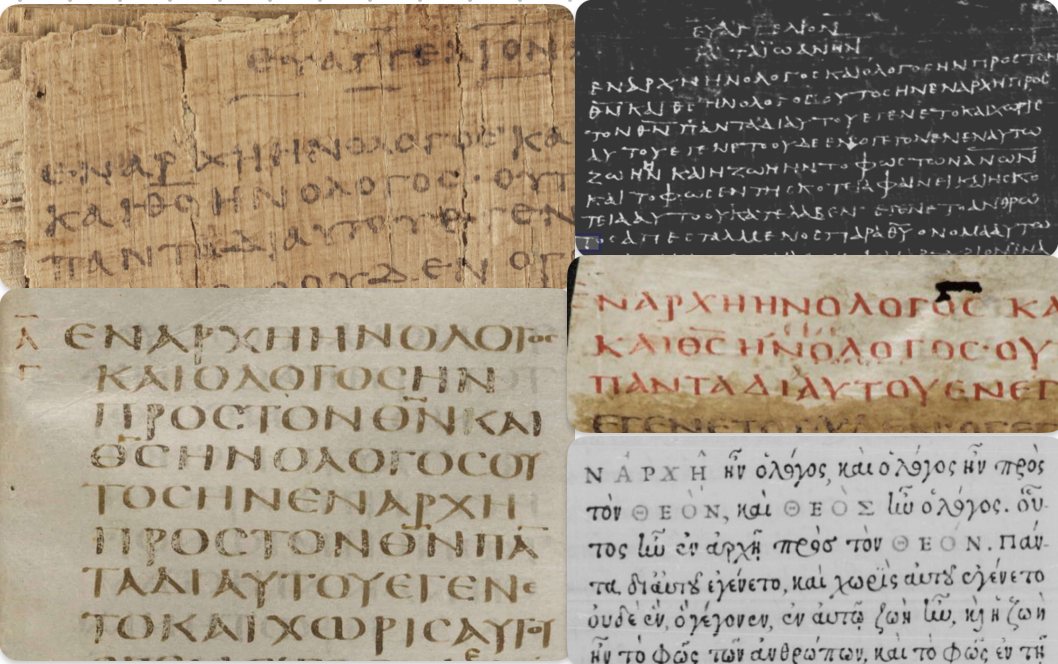
\includegraphics[width=0.5\linewidth]{img/divers_jn_1_1.png}
     \end{figure}
    \vfill
    \pause
    \begin{block}{}
        Dans cette session, nous \textbf{découvrirons un ensemble de témoins du texte néo-testamentaire}.
    \end{block}
\end{frame}

\begin{frame}{Les outils : le NTVMR}


Le NTVMR (New Testament Virtual Manuscript Room):
    \begin{itemize}
        \item Nombreuses numérisations et transcriptions de manuscrits du Nouveau Testament;
        \item Nombreux outils pour la transcription collaborative;
        \item Créé par l'institut pour New Testament Textual Research (Institut für Neutestamentliche Textforschung, INTF).
    \end{itemize}


    \textbf{Accessible à l'adresse} : \url{https://ntvmr.uni-muenster.de}\\

    Le \textit{Manuscript Workspace} permet de consulter des manuscrits et leur transcription en fournissant leur code/nom. 
    \begin{alertblock}{}
        \textbf{Dès que vous voulez vérifier une leçon sur un manuscrit, je vous conseille de vous y rendre directement!} 
    \end{alertblock}

\end{frame}




\section{Codicologie et paléographie du texte néo-testamentaire}

\begin{frame}{Les grandes catégories de manuscrits}
        \begin{alertblock}{}
En critique textuelle néo-testamentaire classique, on sépare \textbf{le texte} (le contenu) de son \textbf{support} (le contenant) afin de l'\textbf{analyser}. 
    \end{alertblock}

    Co-existent donc des classifications:
    \begin{itemize}
        \item Des supports/graphies;
        \item Du contenu des textes sur ces supports.
    \end{itemize}
\end{frame}

\begin{frame}{Les graphies grecques: l'onciale}
\begin{alertblock}{}
    L’\textbf{onciale} est :
    \begin{itemize}
        \item Une graphie particulière des \textbf{alphabets latin, grec et copte};
        \item Utilisée du III\ieme{} au VIII\ieme{} siècle;
        \item Caractérisée par l'absence de liaison entre les lettres;
        \item Qui s'étend entre deux lignes (\emph{bilinéaire}).
    \end{itemize}
\end{alertblock}
\begin{figure}
    \centering
    
\includegraphics[width=0.8\linewidth]{img/majuscule_alphabet.jpg}
\end{figure}
\pause
    \begin{block}{}
        Il s'agit de ce qu'on imagine généralement comme étant \textbf{l'alphabet majuscule}.
    \end{block}
\end{frame}

\begin{frame}{Les graphies grecques: les minuscules}
    \begin{alertblock}{}
        La minuscule grecque est une graphie particulière des alphabets grecques se développant dès le 9\ieme{} siècle, se caractérisant par:
        \begin{itemize}
            \item Un espace entre les mots;
            \item De nombreuses abréviations;
            \item De nombreuses \textbf{ligatures} (lettres se combinant en un nouveau symbole).
        \end{itemize}
    \end{alertblock}

\textbf{Extrait de minuscule 900}:\\

    \centering
    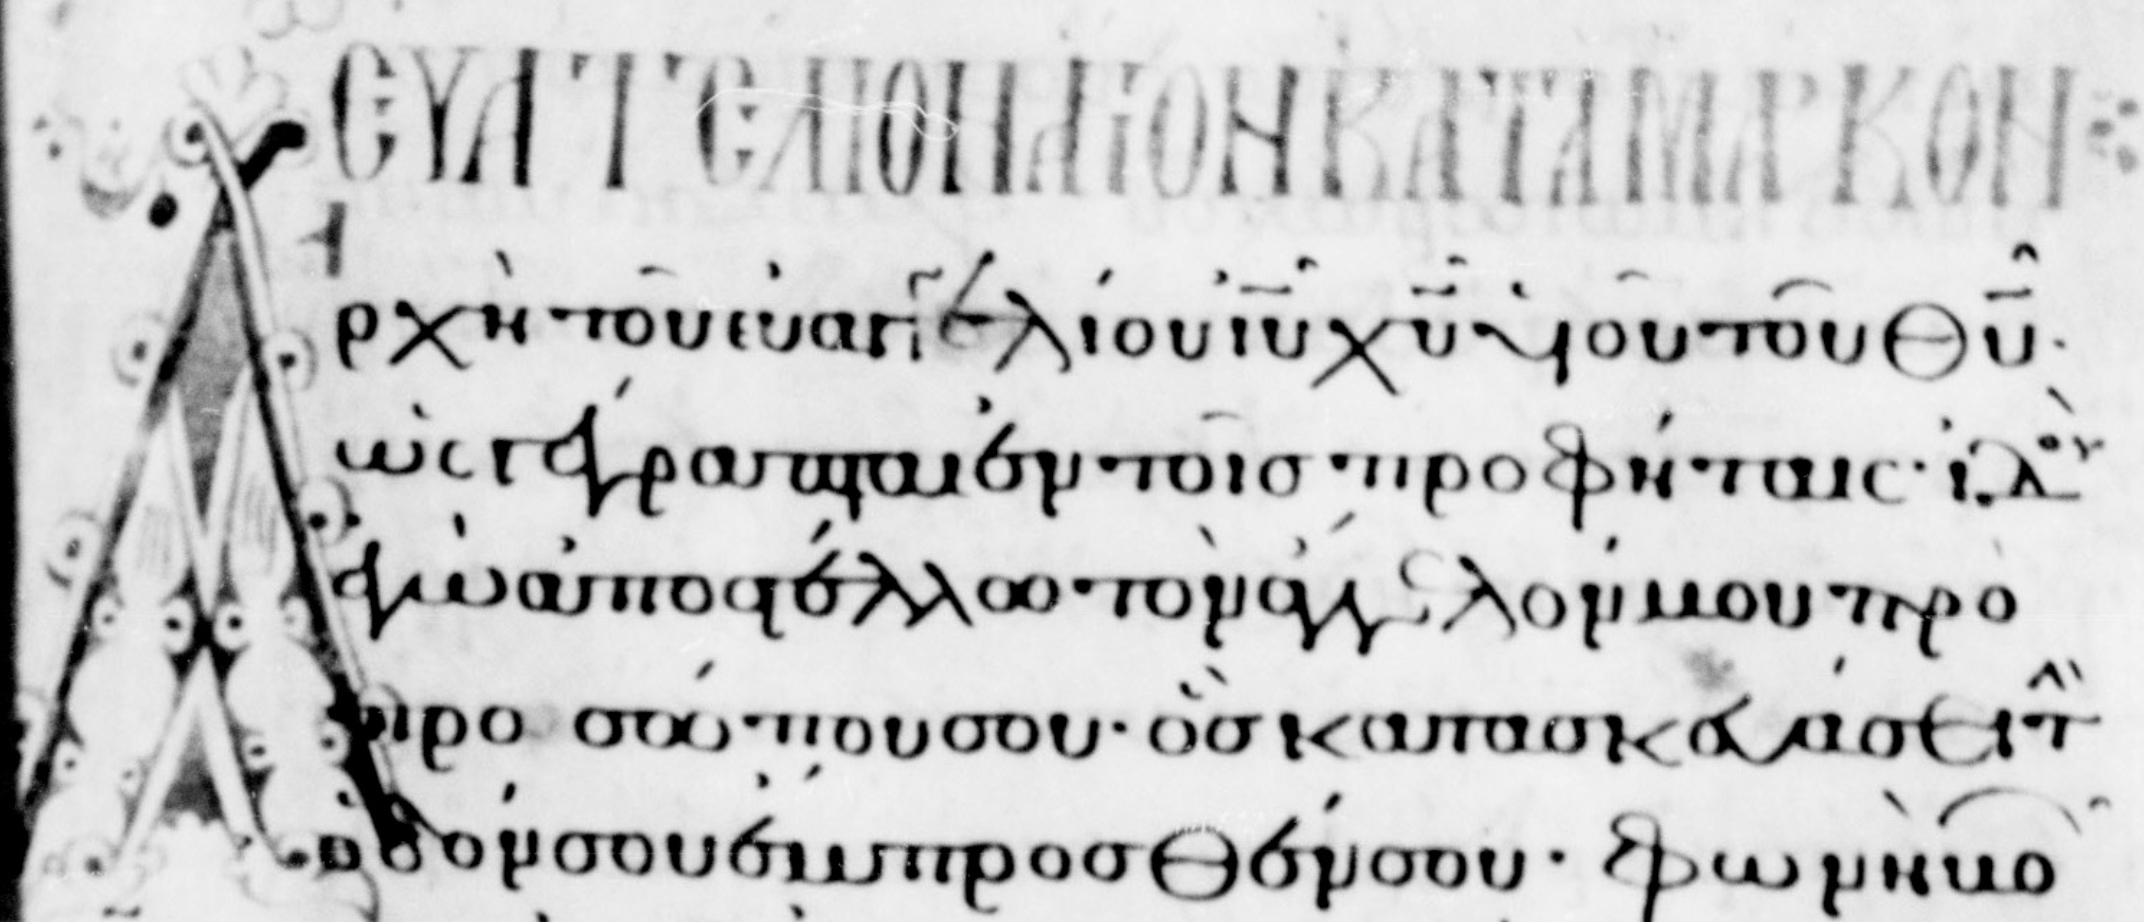
\includegraphics[width=0.5\linewidth]{img/minuscule_900.png}
\end{frame}

\begin{frame}{Les papyri}
    \begin{itemize}
        \item Support d'écriture issu de la superposition de fines lamelles découpées dans la tige de la plante \emph{papyrus};
        \item Attestée dès le -V\ieme{} siècle, en Egypte;
        \item Stocké sous la forme de rouleau;
        \item Décline ensuite à partir du IV\ieme{} siècle, pour être remplacé par le parchemin.
    \end{itemize}
    \begin{alertblock}{}
        Les \textbf{plus anciens témoins textuels} du texte néo-testamentaire sont disponibles forme de papyri (nomenclature $\mathfrak{P}$).
    \end{alertblock}
\end{frame}

\begin{frame}{Les parchemins}
    \begin{itemize}
        \item Support d'écriture issu du traitement de la peau d'animal (mouton, chèvre, veau);
        \item Attesté dès le -II\ieme{} siècle;
        \item Cousu sous la forme d'un codex;
        \item Extrêmement coûteux mais très résistant.
    \end{itemize}

    \begin{alertblock}{}
        Dès le IV\ieme{} siècle, on voit l'utilisation presque exclusive du parchemin.
    \end{alertblock}
\end{frame}

\begin{frame}{Les formes des manuscrits: Le rouleau}
    \begin{itemize}
        \item Consiste en l'enroulage de plusieurs pages collées entre elles (une 20aine en général);
        \item Généralement associé au papyrus, mais il existe des rouleaux de parchemin byzantin.
    \end{itemize}
\end{frame}

\begin{frame}{Les formes des manuscrits : le Codex}
    \begin{itemize}
        \item Ancêtre du livre : couture de plusieurs pages entre elles;
        \item Majoritairement associé au parchemin, mais les codices de papyri ont co-existé;
        \item Popularisé par les chrétiens, \textbf{peut-être en opposition au rouleau considéré comme païen};
    \end{itemize}
\end{frame}

\begin{frame}{Évolution des supports et des graphies}
\begin{figure}
    \centering
    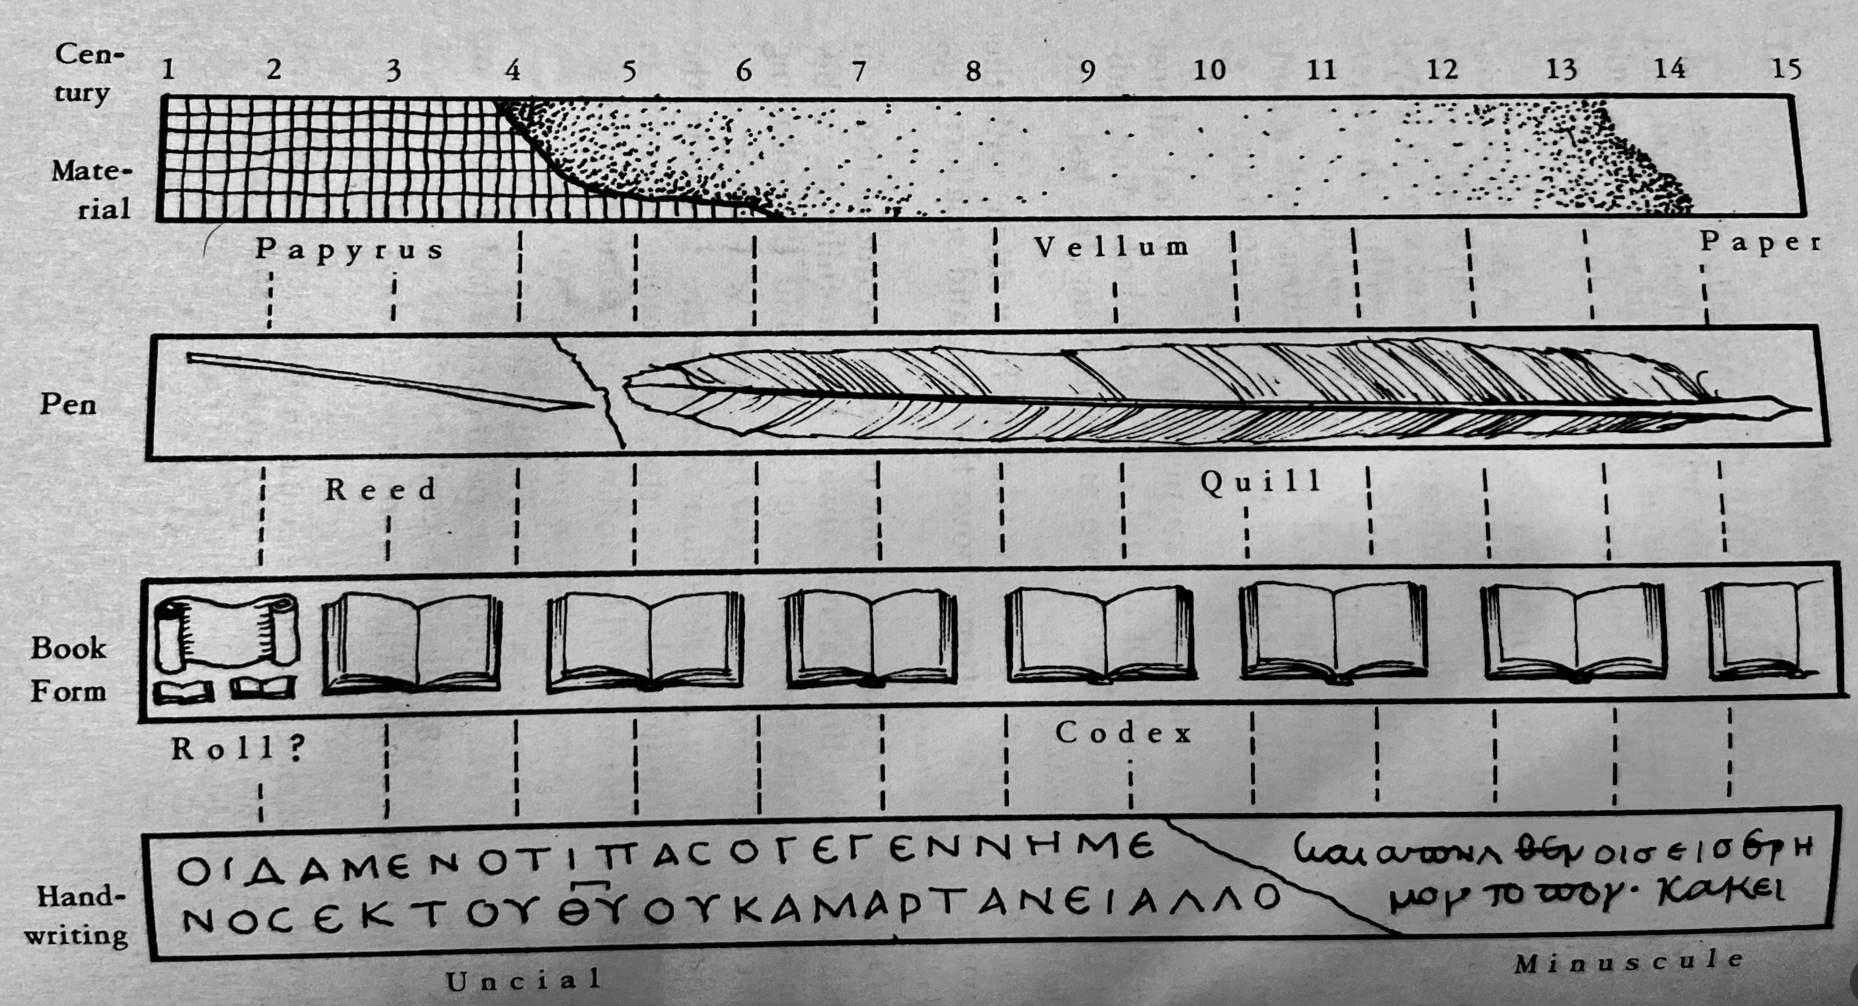
\includegraphics[width=0.5\linewidth]{evolution.png}
\end{figure}
\end{frame}

\section{Les grandes catégories de manuscrit}

\begin{frame}{Les grandes catégories de manuscrits}
\begin{block}{}
    Pouvez-vous proposer une classification des manuscrits distribués \textbf{dans le TP 1 }?
\end{block}
\end{frame}

\begin{frame}{Les grandes catégories de manuscrits}
    La critique textuelle néo-testamentaire \og classique \fg\ divise ses \textbf{sources textuelles} en:
    \begin{enumerate}
        \item Papyri (symbole $\mathfrak{P}$);
        \item Onciaux sur peau (symbole en lettre grecque majuscule);
        \item Minuscules (nombres entiers);
        \item Lectionnaires (\mathcal{l});
        \item Citations patristiques (nom abrégé en minuscule);
        \item Versions du textes néo-testamentaires (nom abrégé en minuscule).
    \end{enumerate}
\end{frame}


\begin{frame}{Les grandes catégories de manuscrits}
    \begin{alertblock}{}
        Pouvez-vous lister ce qui relève de : 
        \begin{itemize}
            \item La paléographie (étude des \textbf{méthodes d'écritures} des manuscrits anciens)
            \item La codicologie (étude du \textbf{support}) ?
            \item Du contenu du texte ?
        \end{itemize}
    \end{alertblock}
\end{frame}




\subsection{Les papyri}


\begin{frame}{Les papyrus}
    \begin{itemize}
        \item Notés avec le signe $\mathfrak{P}$ dans le Nestlé-Aland;
        \item Extrêmement étudié à partir du 20\ieme{} siècle, dû aux nombreuses découvertes archéologiques;
        \item Attestations néo-testamentaires les plus anciennes (par exemple, $\mathfrak{P}^{52} \approx 125$ CE de l'Evangile de Jean);
        \item \textbf{Souvent dans un état fragmentaire}, moins solide que le parchemin.
    \end{itemize}
\end{frame}



\begin{frame}{Le $\mathfrak{P}^{75}$}
\begin{block}{}
    \begin{itemize}
        \item Papyrus fragmentaire daté majoritairement du II\ieme{} siècle;
        \item Luc 3:18–24:53 et nombreux fragments de Jean 1-15;
        \item Très proche du Vaticanus.
    \end{itemize}
\end{block}
    \vfill
\begin{minipage}{.45\textwidth}
\begin{tabularx}{\textwidth}{l|X}
    \small
     Nom & Papyrus 75 ou Papyrus Bodmer XIV–XV \\
     \hline
     Signe & $\mathfrak{P}^{75}$ \\
     \hline
     Code & 10075\\
     \hline
     Date & II\ieme{} au IV\ieme{} \\
     \hline
     Type & Papyrus \\
\end{tabularx}
\end{minipage}
\hfill
\begin{minipage}{.45\textwidth}
    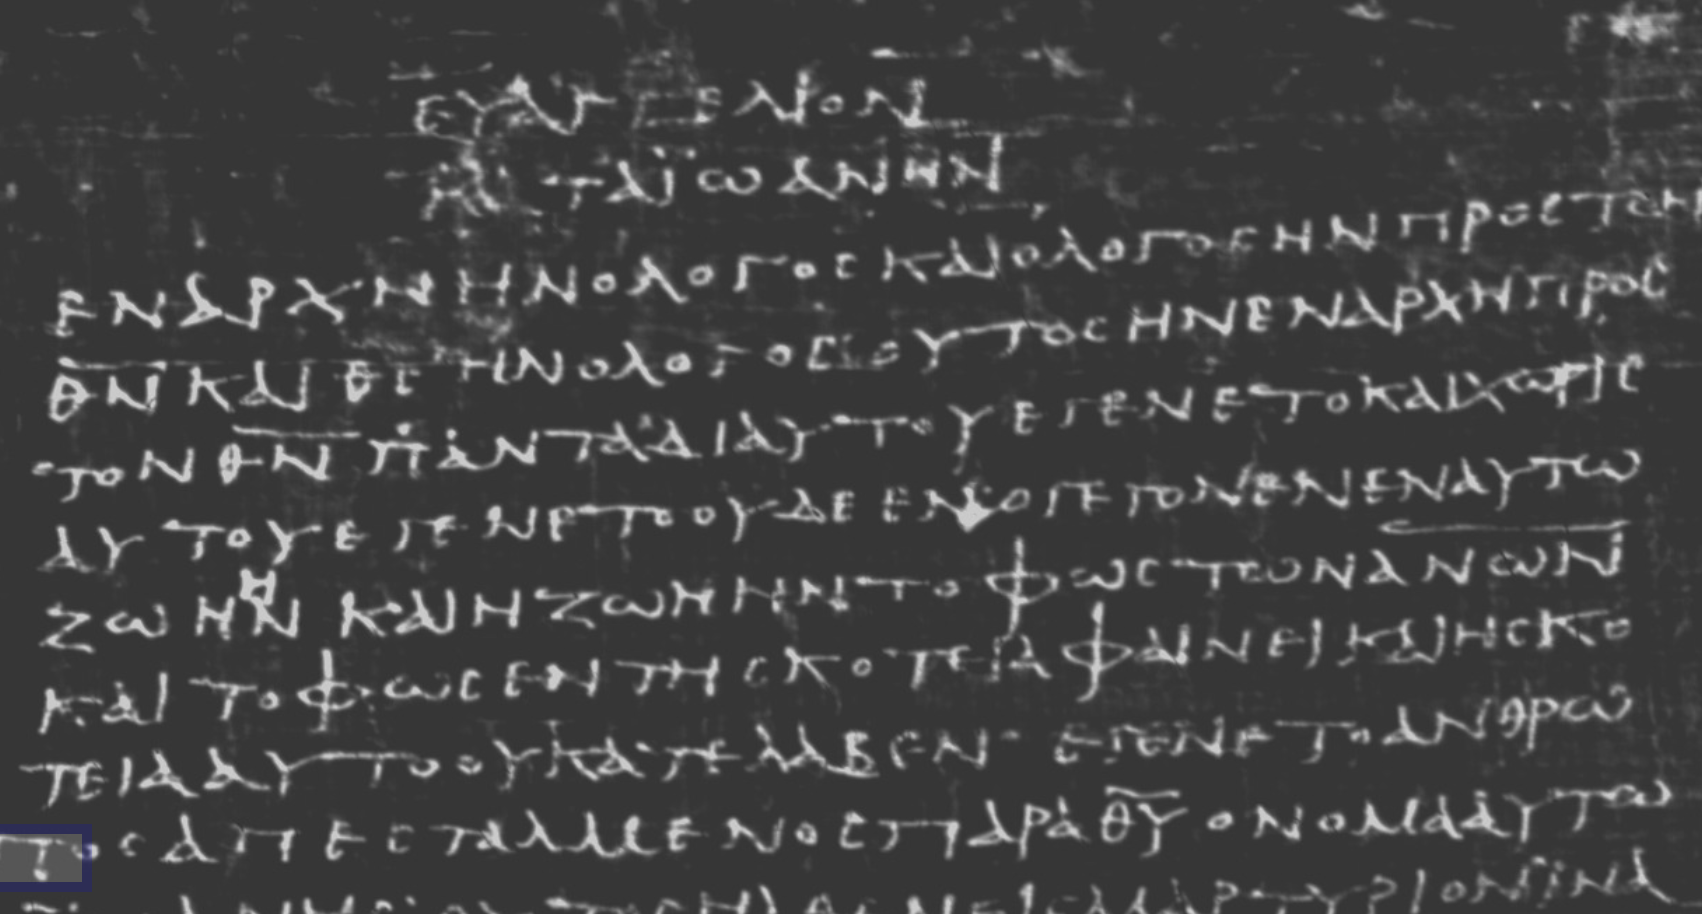
\includegraphics[scale=.2]{img/jn_1_1_p75.png}
\end{minipage}
    
\end{frame}


\begin{frame}{Le $\mathfrak{P}^{75}$}

    \begin{itemize}
        \item Fait partie de la collection \og des \textit{papyrus de Bodmer} \fg\ découvert en 1952;
        \item Énorme implication pour la recherche : le texte est extrêmement proche du Vaticanus, remettant en cause les théories de datation des formes connues des Évangiles > IV\ieme{}.
    \end{itemize}
\end{frame}

\begin{frame}{Le $\mathfrak{P}^{66}$}
    \begin{block}{}
        \begin{itemize}
            \item Préservation exceptionnelle;
            \item La majorité de l'Evangile de Jean : Jean 1:1–6:11; 6:35–14:26,29–30; 15:2–26; 16:2–4,6-7; 16:10–20:20,22–23; 20:25–21:9,12,17.
            \item Présente beaucoup de variantes par rapport au texte standard;
        \end{itemize}
    \end{block}
    \vfill

    \begin{minipage}{.45\textwidth}
\begin{tabularx}{\textwidth}{l|X}
    \small
     Nom & Papyrus Bodmer 2 \\
     \hline
     Signe & $\mathfrak{P}^{66}$ \\
     \hline
     Code & 10066\\
     \hline
     Date & II\ieme{} \\
     \hline
     Type & Papyrus \\
\end{tabularx}
\end{minipage}
\hfill
\begin{minipage}{.45\textwidth}
    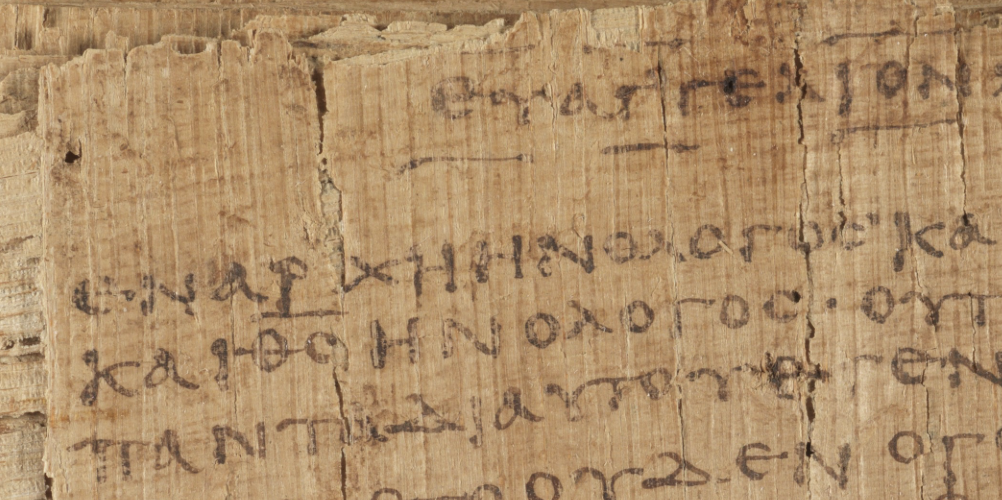
\includegraphics[scale=.4]{img/jn_1_1_p66.png}
\end{minipage}
\end{frame}


\subsection{Les grands codices onciaux}

\begin{frame}{Les onciaux}

    Originellement, \textbf{forme de graphie grecque \og en majuscule \fg}.\\

    
    \pause
    En critique textuelle désigne les grand codices bibliques qui sont:
    \begin{block}{}
        \begin{itemize}
            \item Écrits en oncial;
            \item En \textit{scripto continua} (écriture continue);
            \item \textbf{Contiennent plusieurs livres bibliques regroupés};
            \item Écrit sur des peaux de bonne qualité;
        \end{itemize}
    \end{block}
\end{frame}


\begin{frame}{Les nomina sacra}
    \begin{alertblock}{}
        Le \emph{nomen sacrum} est une manière abrégée pour les scribes de présenter des \textbf{noms avec une signification théologique}.
    \end{alertblock}
\begin{figure}
    \centering
    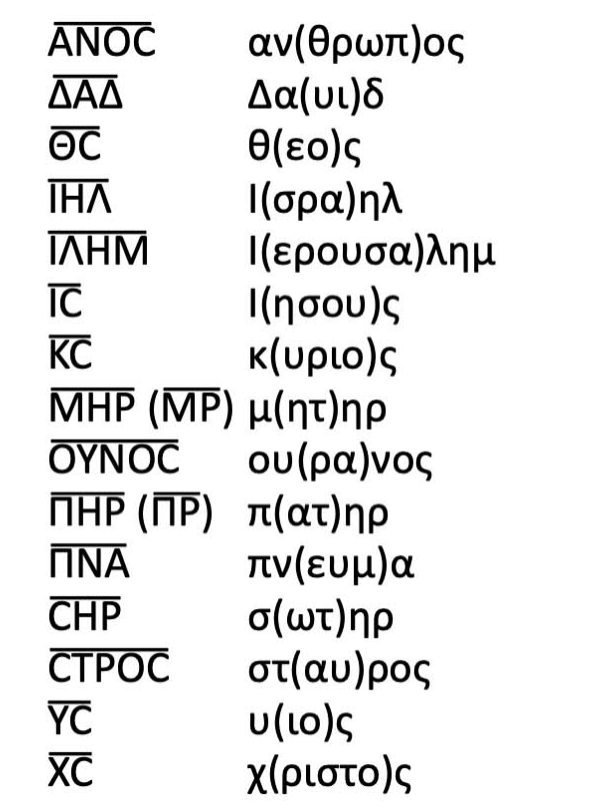
\includegraphics[width=0.3\linewidth]{img/nomen_sacrum.png}
\end{figure}
    
\end{frame}


\begin{frame}{Le Codex Sinaïticus}


\begin{block}{}
    \begin{itemize}
        \item Codex oncial en \textit{scripto continua} qui contient des parties de la Septante et le Nouveau Testament + l'Épître de Barnabé et le Pasteur d'Hermas;
        \item Un des témoins les plus anciens du Nouveau Testament.
    \end{itemize}
\end{block}

    \vfill

\begin{minipage}{.45\textwidth}
\begin{tabular}{l|l}
     Nom & Sinaïticus \\
     \hline
     Signe & $\aleph$ ou $01$ \\
     \hline
     Code & 20001\\
     \hline
     Date & 4\ieme{} siècle, après 325 \\
     \hline
     Type & Oncial \\
\end{tabular}
\end{minipage}
\hfill
\begin{minipage}{.45\textwidth}
    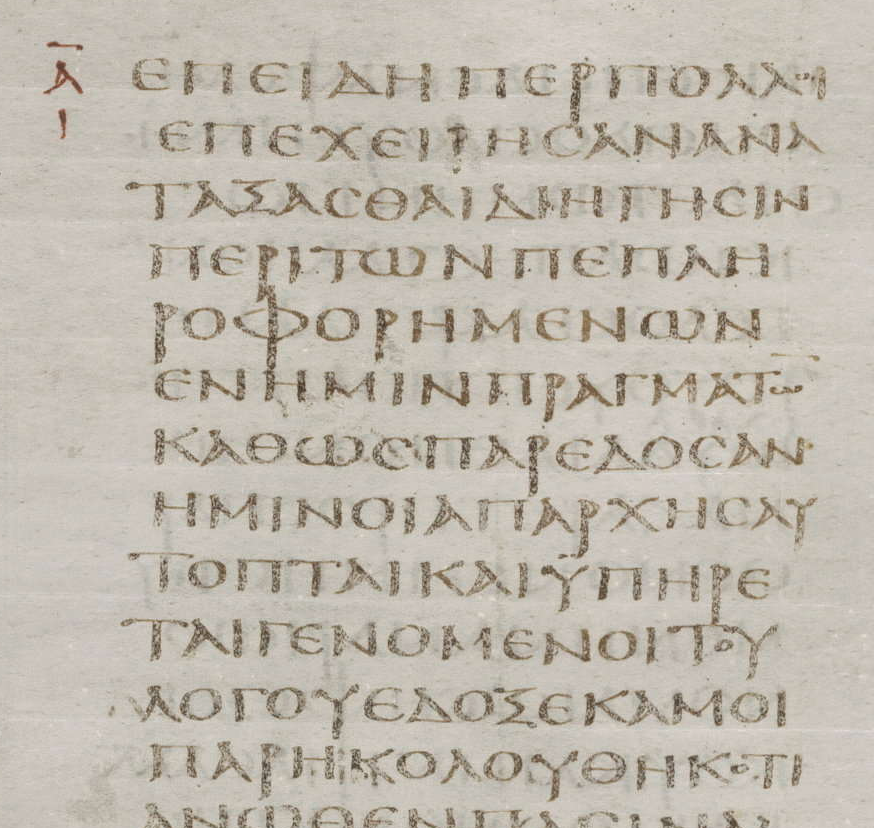
\includegraphics[scale=.2]{img/alexandrinus_luke_inscriptio.png}
\end{minipage}
\end{frame}

% \begin{frame}{Le Codex Sinaïticus}
%     \begin{itemize}
%         \item (Re)-découvert par Constantin von Tischendorf au monastère Sainte-Catherine du Sinaï; 
%         \item Disponible à la British Library, l'université de Leipzig, le monastère Sainte-Catherine du Sinaï, et la Bibliothèque nationale russe;
%         \item Intégralement numérisé en 2005;
%         \item Images et transcriptions disponibles dans leur intégralité sur NTVMR (code 20001).
%     \end{itemize}
% \end{frame}


\begin{frame}{Le Codex Alexandrinus}
\begin{block}{}
    \begin{itemize}
        \item Codex oncial en \textit{scripto continua} qui contient la majorité de la Septante et le Nouveau Testament;
        \item Un des témoins les plus anciens du Nouveau Testament.
    \end{itemize}
\end{block}
    \vfill


\begin{minipage}{.45\textwidth}
\begin{tabular}{l|l}
     Nom & Alexandrinus \\
     \hline
     Signe & $A$ ou 02 \\
     \hline
     Code & 20002\\
     \hline
     Date & 5\ieme{} siècle \\
     \hline
     Type & Oncial \\
\end{tabular}
\end{minipage}
\hfill
\begin{minipage}{.45\textwidth}
    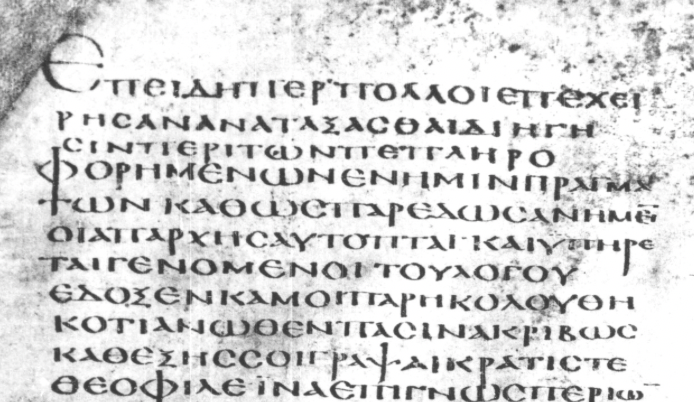
\includegraphics[scale=.4]{img/alexandrinus_lk_11.png}
\end{minipage}

\end{frame}

% \begin{frame}{Le Codex Alexandrinus}

% \begin{itemize}
%     \item Tire son nom d'Alexandrie où l'on suppose qu'il fut rédigé (on cite également la Palestine);
%     \item Propriété du Patriarche d'Alexandrie depuis 1098, donné à Charles Ier d'Angleterre en 1628 par le patriarche oriental Cyrille Louokaris et conservé à la \emph{Bristish Library};
%     \item De \textbf{nombreuses corrections} réalisés par des mains postérieures.
% \end{itemize}
    
% \end{frame}

\begin{frame}{Le Codex Vaticanus}
    \begin{block}{}
    \begin{itemize}
        \item Codex oncial en \textit{scripto continua} qui contient la majorité de la Septante et le Nouveau Testament;
        \item Un des témoins sous forme de codex les plus anciens du Nouveau Testament.
    \end{itemize}
\end{block}


\begin{minipage}{.45\textwidth}
\begin{tabular}{l|l}
     Nom & Vaticanus \\
     \hline
     Signe & $B$ ou 03 \\
     \hline
     Code & 20003\\
     \hline
     Date & 4\ieme{} siècle \\
     \hline
     Type & Oncial \\
\end{tabular}
\end{minipage}
\hfill
\begin{minipage}{.45\textwidth}
    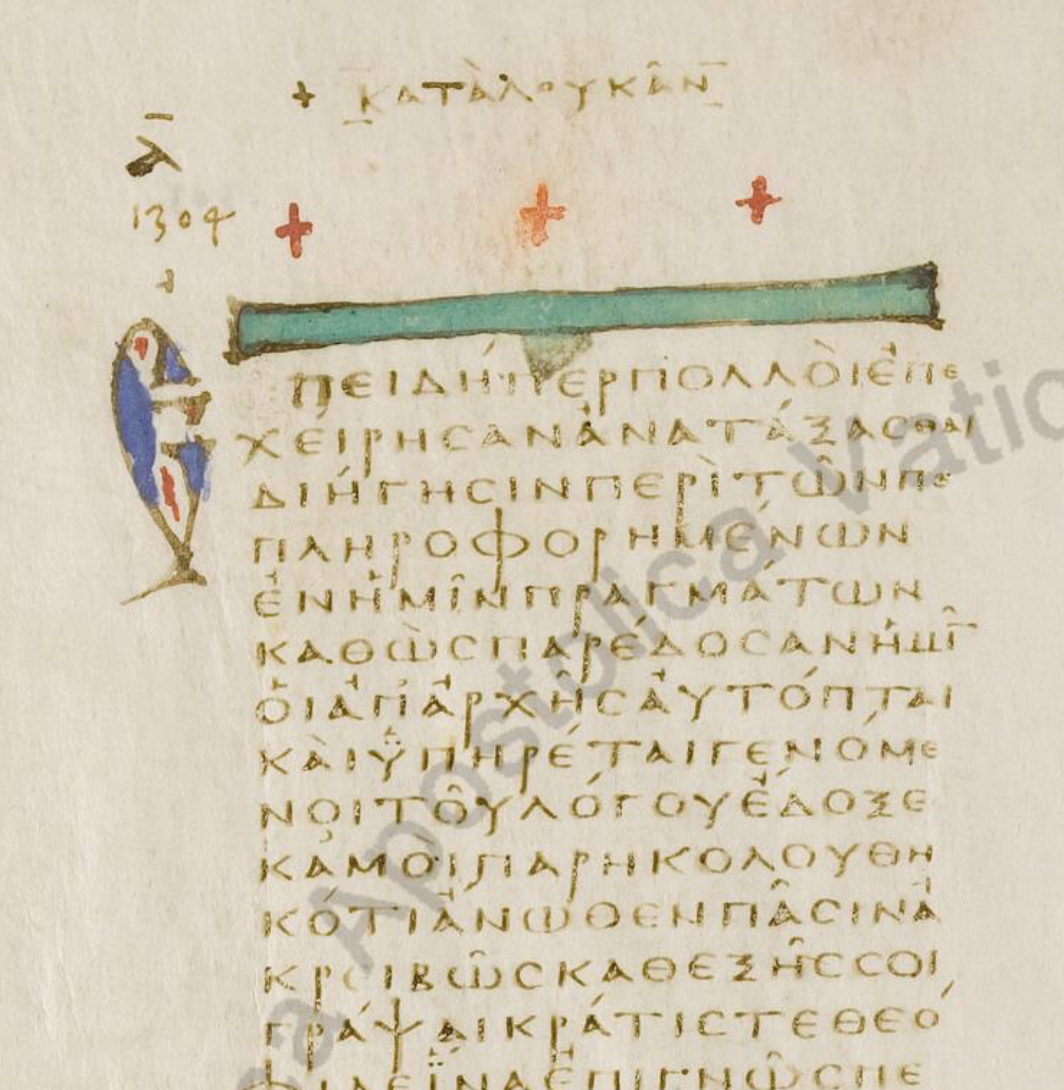
\includegraphics[scale=.2]{img/vaticanus_luke_inscriptio.png}
\end{minipage}
\end{frame}

% \begin{frame}{Le Codex Vaticanus}
% \begin{itemize}
%     \item Ré-encré au Moyen-Age;
%     \item N'a peut-être jamais quitté l'Italie (recensé en 1475 par la bibliothèque Vaticane);
%     \item Initialement peu utilisé par la critique textuelle renaissante (par Erasme);
%     \item Intérêt renouvelé au 19\ieme{};
%     \item \textbf{Aujourd'hui considéré comme étant un des témoins principaux du texte néo-testamentaire}.
% \end{itemize}
    
% \end{frame}


\begin{frame}{Le Codex Bezae}
    \begin{block}{}
        \begin{itemize}
            \item Codex oncial en \textit{scripto continua};
            \item Contient les 4 Évangiles, les Actes et une partie de la troisième épître de Jean;
            \item Recto en grec, verso en latin;
            %\item Écrit dans une très belle encre rouge.
        \end{itemize}
    \end{block}
        \vfill
    \begin{minipage}{.4\textwidth}
\begin{tabular}{l|l}
     Nom & Bezae \\
     \hline
     Signe & $D$ ou 05 \\
     \hline
     Code & 20005\\
     \hline
     Date & V\ieme{} siècle \\
     \hline
     Type & Oncial \\
\end{tabular}
\end{minipage}
\hfill
\begin{minipage}{.45\textwidth}
    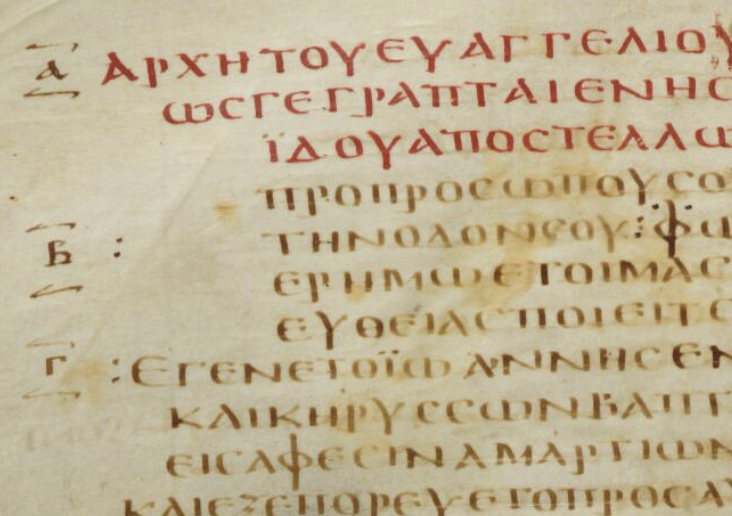
\includegraphics[scale=.4]{img/bezae_mk_1_1.png}
\end{minipage}
\end{frame}

% \begin{frame}{Le Codex Bezae}
%     \begin{itemize}
%         \item \textbf{Nombreuses variantes textuelles} par rapport aux autres textes;
%         \item Propose \textbf{un ordre des Évangiles différents} (Matthieu - Jean - Luc - Marc);
%         \item Peut être originaire de la Gaule (actuelle France) ou du sud de l'Italie. D'autres endroits suggérés incluent l'Égypte, la Palestine et Beyrouth.

%         \item Manuscrit longtemps gardé dans la bibliothèque monastique de Saint Irénée à Lyon.
%         \item Vol lors des guerres de Religion au XVIe siècle par des Huguenots français en 1562 et \textbf{remis à Thédore de Bèze}. En 1581, il a été donné à l'Université de Cambridge, en Angleterre.
%     \end{itemize}
% \end{frame}

\subsection{Les minuscules}

\begin{frame}{Les minuscules}
Par abus de langage, désigne les textes du Nouveau Testament rédigé avec la calligraphie minuscule.
\pause
\begin{block}{}
    \begin{itemize}
        \item Texte les plus récents;
        \item \textbf{Énormément de témoins, travaux de référencement et de transcription encore en cours} !
        \item Majoritairement utilisées pour les travaux de critique textuelle du XVI\ieme{} mais \dots
        \item ... \og négligées \fg\ de la critique textuelle du XX\ieme{}.
    \end{itemize}
\end{block}

\end{frame}

\begin{frame}{Minuscule 33}
        \begin{block}{}
        \begin{itemize}
            \item Majorité de l'Ancien et du Nouveau Testament (sauf l'Apocalypse);
            \item Témoin très utilisé en critique textuelle.
        \end{itemize}
    \end{block}
    \vfill
    \begin{minipage}{.45\textwidth}
\begin{tabularx}{\textwidth}{l|X}
    \small
     Nom & Minuscule 33 \\
     \hline
     Signe & 33 \\
     \hline
     Code & 30033\\
     \hline
     Date & IX\ieme{} \\
     \hline
     Type & Minuscule \\
\end{tabularx}
\end{minipage}
\hfill
\begin{minipage}{.45\textwidth}
    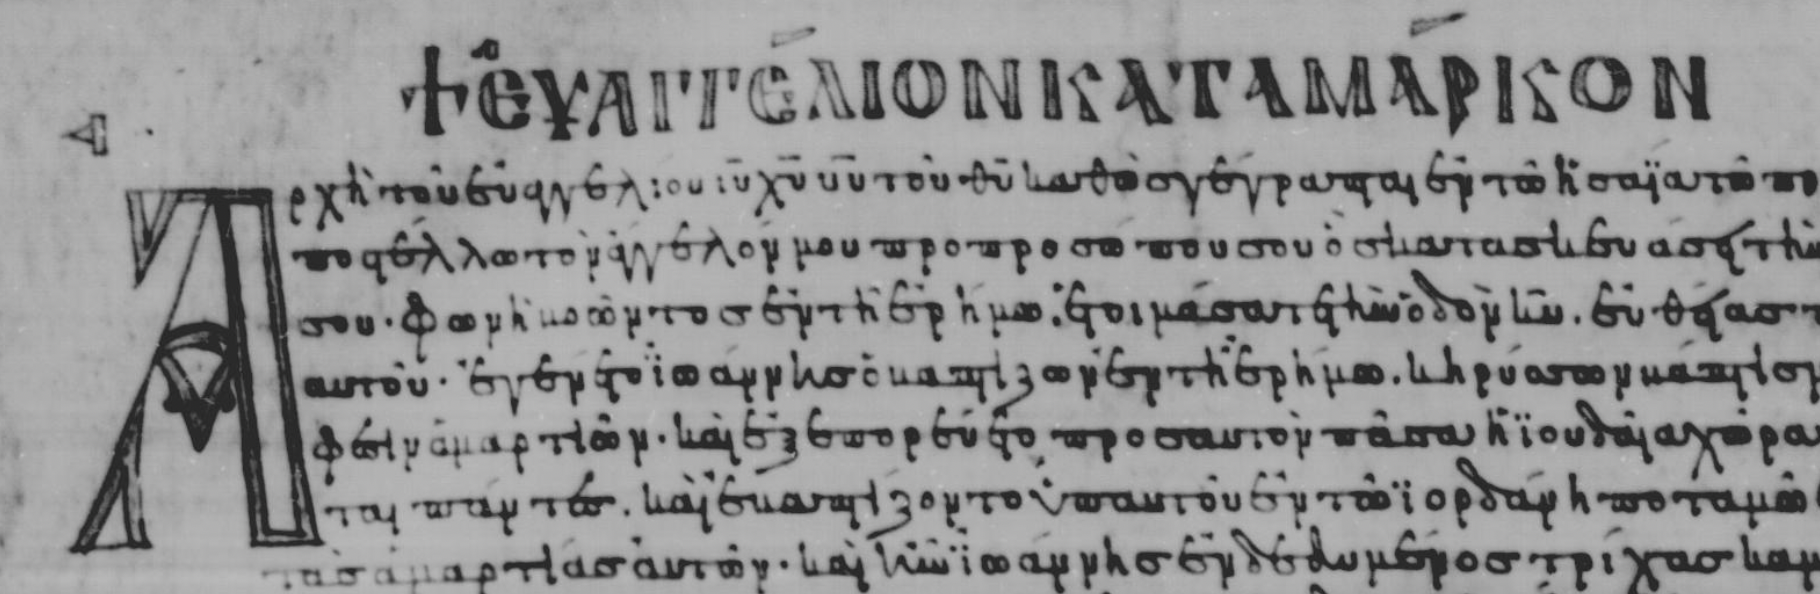
\includegraphics[scale=.16]{img/minuscule33.png}
\end{minipage}
\end{frame}

\subsection{Autres formes de texte}

\begin{frame}{Les lectionnaires}
\begin{minipage}{.5\textwidth}
    \begin{itemize}
        \item Texte biblique segmenté en fonction du calendrier liturgique;
        \item Noté par ℓ dans la classification d'Aland (préfixé de 40 dans le NTVMR);
    \end{itemize}
\end{minipage}%
\hfill
\begin{minipage}{.4\textwidth}
ℓ 183 (40183):\\

    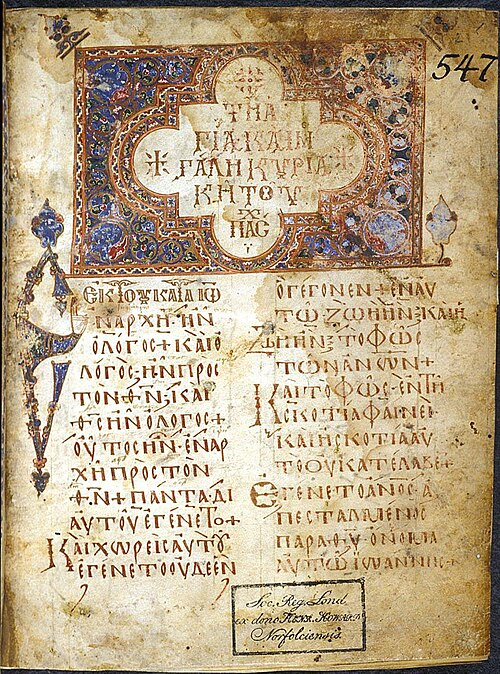
\includegraphics[scale=.2]{img/Lectionary_183_folio_2.JPG}
\end{minipage}

\end{frame}

\begin{frame}{Les citations patristiques}
\begin{itemize}
    \item Nombreuses citations du texte biblique par les Pères de l'Eglise;
    \item Notamment dans les commentaires suivis (Origène \dots)
    \item \textbf{Travail très long de collection et d'analyse}.
\end{itemize}
    
\end{frame}

\section{Les versions du Nouveau Testament}

\begin{frame}{Les versions du Nouveau Testament}
    \textbf{Dès l'avènement du christianisme, le Nouveau Testament a été traduit en de multiples langues antiques}.

    \begin{block}{}
        Pouvez-vous citer quelques unes de ces langues ?
        \pause
        \begin{itemize}
            \item Latin;
            \item Syriaque;
            \item Copte;
            \item Gothique;
            \item Arabe \dots
        \end{itemize}
    \end{block}
    \pause
    
    \begin{alertblock}{}
La présence de toutes ces différentes versions compliquent encore \textbf{les schémas de transmission du texte}.
    \end{alertblock}
\end{frame}

\begin{frame}{Les versions latines}
    2 versions latines majeures du Nouveau Testament :

    \begin{enumerate}
        \item \textbf{Les Vieilles Latines} (\textit{Itala}, OL) : ensemble de traductions en latin (2 \ieme{} siècle (?) - 9\ieme{} siècle), présentant un latin peu raffiné et une grande multiplicité textuelle. \textbf{Environ 30 manuscrits}.\\
        \textbf{Exemple} : le latin du Codex de Bèze.\\
        \pause
        
        \item \textbf{La Vulgate} : face à la multiplicité des vieilles latines, en 382 Jérôme est mandaté de réaliser une version standardisée, qui sera ré-éditée au concile de Trente (Sixtine et Clémentine). \textbf{Environ 8000 manuscrits}.\\
    \end{enumerate}
\end{frame}

\begin{frame}{Les versions syriaques}
    \begin{alertblock}{}
    Le \textbf{syriaque} est une langue sémitique très proche de l'araméen (langue de Jésus ?), parlée aux alentours de la Palestine.
    \end{alertblock}
    \pause
    
    Plusieurs versions du texte syriaque:
    \begin{itemize}
        \item Le Diatessaron (harmonie des Évangiles), attribuée à Tatien (160). \textbf{Aucun manuscrit}.
        \item La vieille syriaque (fin du 2\ieme{} siècle, évangiles). \textbf{2 manuscrits}.
        \item La Peschitta (5\ieme{} siècle), version standardisée encore en vigueur. \textbf{250 manuscrits}.
        \item Le syriaque philoxenien. \textbf{2 manuscrits}.
        \item Le syriaque harkléien. \textbf{50 manuscrits}.
        \item Le syriaque paléstinien. Lectionnaire très proche du grec. \textbf{2 manuscrits}.
    \end{itemize}
\end{frame}

\begin{frame}{Les versions coptes}
\begin{alertblock}{}
    Le copte est une langue chamito-sémitique issue de \textbf{l'égyptien ancien}, dérivée de l'égyptien démotique avec l'alphabet du grec ancien auquel on a ajouté des caractères du démotique.
\end{alertblock}
\centering
    
\includegraphics[width=\linewidth]{exemple_copte.png}
\flushleft
Plusieurs dialectes:
\begin{itemize}
    \item Sahidique;
    \item Boharique.
\end{itemize}
\end{frame}

\begin{frame}{Autres versions}
Autres versions du texte:
    \begin{itemize}
        \item Arménien;
        \item Géorgien;
        \item Ethiopien;
        \item Arabe;
        \item Slave;
        \item Slavon.
    \end{itemize}
\end{frame}

% \begin{frame}{Les versions du Nouveau Testament}
%     \begin{itemize}
%         \item Deux versions \textbf{latines} (\emph{latt}) : 
%         \begin{itemize}

%             \item Vulgate (\emph{vg})
%             \item Vetus Latina (OL ou \emph{it} ou \textit{f ff1});
%         \end{itemize}
%         \pause
%         \item Versions \textbf{coptes} (\emph{ac, bo, mae, mf, pbo, sa}):
%         \begin{itemize}
%             \item Sahidique;
%             \item Bohairique.
%         \end{itemize}
%         \pause
%         \item Versions \textbf{syriaques} (dialecte de l'araméen), \emph{syr} :
%         \begin{itemize}
%             \item Diatessaron (Harmonie des Évangiles)
%             \item Vieille Syriaque (Evangiles);
%             \item Peshitta (Texte vétéro et néo-testamentaire).
%         \end{itemize}
%     \end{itemize}
% \end{frame}



\section{Classifier le texte du Nouveau Testament}

\begin{frame}{Les textes du Nouveau Testament}

    \begin{alertblock}{}
En critique textuelle néo-testamentaire classique, on sépare \textbf{le texte} (le contenu) de son \textbf{support} (le contenant) afin de l'analyser. 
    \end{alertblock}

    Il y a alors une classification du \textbf{texte} (plutôt que du support comme nous venons de le voir).
\end{frame}

\begin{frame}{Les textes grecs}
    Classification classique et en vigueur chez les textualistes "classiques" (\textbf{à prendre avec du recul}) :

    \begin{itemize}
        \item \textbf{Alexandrin} : texte neutre, le plus proche de \og l'original \fg.\\ \textbf{Témoins principaux} : $\aleph$, B, $\mathfrak{P}^{75}$.
        \item \textbf{Occidental} : beaucoup de variants, variation dans le texte des Actes. \\
        \textbf{Témoin principal} : D.
        \item \textbf{Byzantin} : considéré comme raffiné à la fin de l'Antiquité, présentant beaucoup d'harmonisation et une bonne qualité littéraire;
        \item \textbf{Césaréen} (?) : existence remise en cause par les chercheurs, texte intermédiaire entre l'Alexandrin avec quelques influences byzantines. \\
        \textbf{Témoins principaux} : $f^1$, $f^{13}$.
    \end{itemize}
\end{frame}

\subsection{La classification des manuscrits par Aland}

\begin{frame}{Classification des manuscrits}
En plus de leur classification par support, classification en fonction de \og \textbf{qualité} \fg\ (\textit{terme à prendre avec beaucoup de recul !!!}) :
\pause
\begin{itemize}
\item \textbf{Catégorie I} : Manuscrits très anciens et peu influencés par le texte byzantin.
\pause

\item \textbf{Catégorie II} : Manuscrits similaires à la Catégorie I mais avec quelques influences étrangères.
\pause

\item \textbf{Catégorie III} : Manuscrits avec un texte distinctif, important pour l'histoire textuelle.
\pause

\item \textbf{Catégorie IV} : Manuscrits suivant le texte du Codex Bezae (D), de type occidental.
\pause

\item \textbf{Catégorie V} : Manuscrits avec un texte principalement byzantin.
\pause

\item \textbf{Non classés} : Manuscrits qui ne rentrent pas clairement dans une catégorie.
\end{itemize}
\end{frame}

\begin{frame}{Questions}
    Questions ?
\end{frame}

\end{document}